Vi har valgt at analysere vores project i forhold bohms model, samt at lave risici analyse p� forskellige muligheder mht. teknologi heriblandt: Android og Windows mobile, eventuelt kunne vi ogs� have overvejet mobile web. For hver enkelt teknologi skal overvejes specielt i forhold vores erfaring med den, samt relevans ift. m�let. \\

\subsection*{Bohms model}
% efterf�lgende skal opdateres
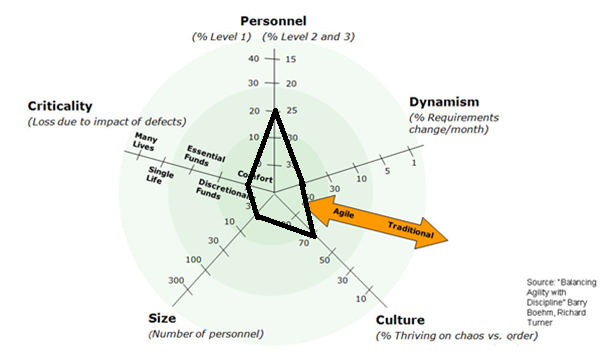
\includegraphics[scale=1.00]{includes/billeder/bohmsmodel.png} \\
Vi en lille gruppe p� 3, med kun 2 udviklere. Det er ikke kritisk om hvorvidt appen skulle crashe s� vi har vurderet Criticality til Comfort. For Personnel har vi vurderet til at ligger cirka midt p� idet at vi har meget forskelligt fagligt niveau i forhold til kodning. Vi forventer at der bliver brug for meget dynamik, idet at vi har lidt kendskab til teknologierne og at der derfor h�jst sandsynligt vil opst� en masse �ndringer undervejs i processen. I gruppen trives vi med en lille smule overordnet planl�gning, men ellers p� kaos og h�j personlig frihed. 

\begin{center}
\line(1,0){450}
\end{center}

\subsection*{Risici analyse}
Vi har valgt at fokusere p� risici for Android og Windows mobile idet at vi mener at disse er blandt de mest relevante teknologier i forhold til vores app. Yderligere kunne man evt. vurdere for IPhone og mobile web.

\subsubsection*{Android mobile}
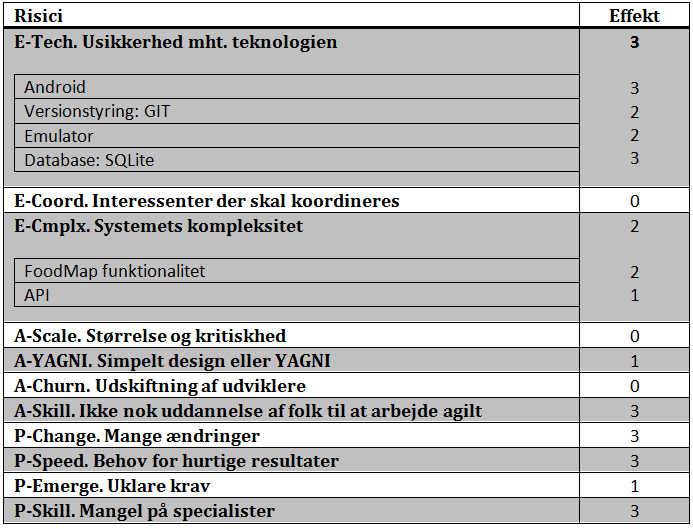
\includegraphics[scale=0.70]{includes/billeder/risici_analyse_android.png} \\ \\

\textsf{Omgivelser (Enviroment):} \\
Vi har vurderet at der er h�j usikkerhed mht. teknologien specielt ift. Android og SQLite. Der er ikke nogen interessenter der skal koordineres. Systemets kompleksitet vil have en moderat effekt, mest er det FoodMap funktionaliteten som kan vise sig problematisk da vi ikke helt ved hvad den indeb�rer, samt at der vil forekomme nogle performance og usability krav der hurtigt kan g�re systemet komplekst. \\ 
\textsf{Effekt point ialt:}
3 + 0 + 2 = 5
\\ \\


\textsc{Agile A-risici:} \\
Umiddelbart er det er et relativt sm�t projekt, derfor har vi vurderet A-Scale til ikke at have nogen effekt. Simpelt design vil ikke have den store effekt, da der ikke beh�ves den store planl�gning eller dokumentation af systemet. Der vil ikke v�re nogen udskiftning af udviklere s� A-Churn har ingen effekt. A-Skill kan g� hen at f� en stor effekt, idet at vores uddannelsesniveau er meget lavt i forhold til teknologien. \\ \\    
\textsf{A-risici ialt:} \\ 
0 + 1 + 0 + 3 = 4 \\ \\

\textsc{Plan-driven P-risks:} \\
Vi forventer at der vil forekomme mange �ndringer og dette vil have en stor effekt. Derudover er der et behov for hurtige resultater, idet at vi har brug for l�bende releases for at f� feedback fra reviews. Uklare krav vil have en meget lille effekt, idet at det i h�j grad er os selv der definerer dem. Mangel p� specialister vil have en stor effekt, da specialiser er n�dvendige for at kunne bruge de plandrevne v�rkt�jer ordentligt med den p�g�ldende teknologi. \\
\textsf{P-risks ialt:} \\
3 + 3 + 1 + 3 = 10

%\begin{itemize}
%\item E-Tech. Usikkerhed mht. teknologien: 2 
%\begin{itemize}
%\item Android ide: 2
%\item Versionstyring: 3
%\item Emulator: 1
%\end{itemize}
%
%\item E-Coord. Interessenter der skal koordineres: 0
%\item E-Cmplx. Systemets kompleksitet: 2
%\begin{itemize}
%\item FoodMap funktionalitet: 2
%\item API: 1
%\end{itemize}
%
%\item A-Scale. St�rrelse og kritiskhed: 0
%\item A-YAGNI. Simpelt design eller YAGNI: 1
%\item A-Churn. Udskiftning af udviklere: 0
%\item A-Skill. Ikke nok uddannelse af folk til at arbejde agilt: 3
%\item P-Change. Mange �ndringer: 1
%\item P-Speed. Behov for hurtige resultater: 2
%\item P-Emerge. Uklare krav: 1
%\item P-Skill. Mangel p� specialister: 3
%\end{itemize}

\begin{center}
\line(1,0){450}
\end{center}

\subsubsection*{Windows mobile} 
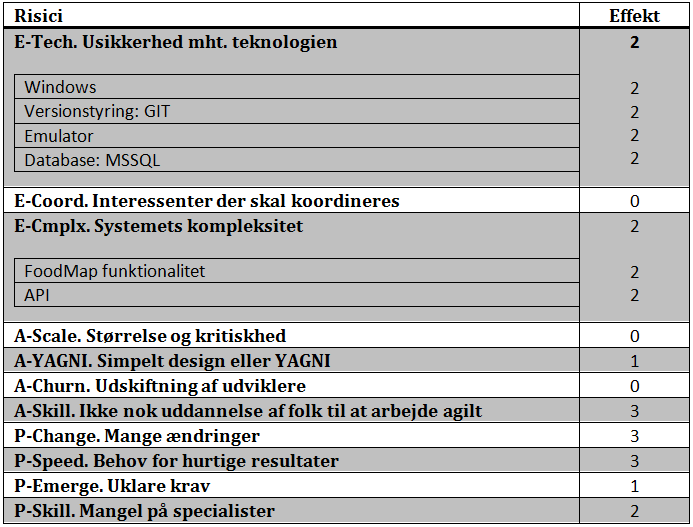
\includegraphics[scale=0.70]{includes/billeder/risici_analyse_windowsphone.png} \\


\textsf{Omgivelser (Enviroment):} \\
Vi har vurderet at der er j�vn usikkerhed mht. teknologien idet at vi ikke den store viden for Windows mobile, dog har vi tidligere erfaring med Visual studio og MSSQL. Der er ikke nogen interessenter der skal koordineres. Systemets kompleksitet vil have en moderat effekt, mest er det FoodMap funktionaliteten som kan vise sig problematisk da vi ikke helt ved hvad den indeb�rer, samt at der vil forekomme nogle performance og usability krav der hurtigt kan g�re systemet komplekst. \\ \\
\textsf{Enviroment effekt ialt:} \\
2 + 0 + 2 = 4 \\ \\

\textsc{Agile A-risici} og \textsc{Plan-driven P-risks:} \\
Umiddelbart er vilk�rene de samme som for Android mobile, men idet at vi har arbejdet mere med .NET, Visual studio og MSSQL forinden har vi valgt at vurdere effekten p� P-Skill lavere. \\
\textsf{A-risici ialt:} \\
0 + 1 + 0 + 3 = 4 \\

\textsf{P-risks ialt:} \\
3 + 3 + 1 + 2 = 9

\subsection*{Metodevalg}
Da vi er en lille gruppe som har det bedst med at der ikke er en for stram process og meget personlig frihed under ansvar, foretr�kker vi en meget agil udviklingsmetode og process. \\
Man m� ud fra vores risici-analyse konkludere at vi har meget usikkerhed med teknologien og at det derfor vil v�re en god ide at s�rge for at f� noget kvalitetssikring ind over udviklingen, gerne i form af unit testing.
Det ser umiddelbart ud som om at Windows mobile er nemmere at tilg�, men idet at Android markedet har flere brugere, finder vi det mere relevant at arbejde med.